\chapter{Experiments and results}
\label{experiments_and_results}

The algorithm presented in this work was implemented and several experiments with a simple garment dataset were conducted. This chapter is devoted to explain the experiments performed using the algorithm presented in this thesis. It includes the implementation details, the experimental setup and the experiments themselves, as well as the results obtained through those experiments.

\section{Implementation details}
\label{experiments:implementation}
The software implementation for this thesis has two main parts. The first one is in charge of communication with the sensor with the objective of extracting the depth data. This communication is performed using YARP \reftodo. YARP is a set of libraries, protocols, and tools that leverages many common tasks required for a humanoid robot to work. Those tasks include actuator control and command, communications with the robot and between software parts, and accessing to data captured from different common sensors, such as depth sensors.

The second one is the implementation of the unfolding algorithm. This implementation was executed using Python\footnote{\url{http://www.python.org}} as our language of choice. Python is a programming language that allows a quick development of prototype software, and that counts with a large collection of external modules to perform several tasks, from math calculations to computer vision. Our implementation is based on tho different computer vision libraries: OpenCV\footnote{\url{http://www.opencv.org}} and Scikit-image\footnote{\url{http://scikit-image.org}}. We chose to use both since during the development of this work several algorithms were evaluated, and each library contains only a subset of those algorithms. In the latest version, OpenCV is used for basic computer vision and Scikit-image for more advanced algorithms such as Watershed \footnote{\url{http://scikit-image.org/docs/dev/auto_examples/plot_watershed.html}} and other superpixel-based clustering methods. 

The whole unfolding algorithm implementation is Open Source, and is available online\footnote{\url{https://github.com/roboticslab-uc3m/textiles}}.

\section{Experimental Setup}
\label{experiments:expermimental_setup}

The experimental setup consisted of several elements in a laboratory environment: a table, a depth sensor and a humanoid robot. The garment was placed on a white, flat surface, parallel to the floor. Over the garment, an ASUS Xtion PRO LIVE depth sensor was attached to a structure to capture data from a top view. The unfolding operation was performed by our full-body humanoid robot TEO \cite{martinez2012teo}. Figure \ref{fig:experimental_setup} depicts this setup.

\begin{figure}[thpb]
    \centering
    
\includegraphics[width=0.7
    \textwidth]{figures/placeholder2.png}
    \caption{\comment{Here I should put a nice figure of the experimental setup}}
    \label{fig:experimental_setup}
\end{figure}

The starting point for testing our algorithm is the data adquisition process. Data is obtained as a point cloud from a ASUS Xtion Pro Live sensor. Then, it is converted to a depth map image for its later analysis. 

This conversion is done by simply using the z component of each point as the depth value for each pixel of the depth image. If there were a known deviation from the surface (affecting perpendicularity), the depth image could be recovered from the point cloud using the instrinsic and extrinsic parameters of the sensor instead. As the sensor is placed on top of the garment, perpendicular to the surface on which the clothing article rests, both methods yield very similar results, as shown in figure \ref{fig:point_cloud_and_depth_image}.

\begin{figure}[thpb]
    \centering
    
\includegraphics[width=0.7
    \textwidth]{figures/placeholder2.png}
    \caption{\comment{Here I should put a nice figure of the point cloud and the depth image}}
    \label{fig:point_cloud_and_depth_image}
\end{figure}

The RGB values are also recorded for each depth image, obtaining an RGB-D image.

\section{Experiments}
\label{experiments:experiments}

The final experiments using the current algorithm have been performed using an ASUS Xtion PRO LIVE at 640x480 RGB and depth streams (30 fps).

In the present work we are using thick blankets and towels, to cope with the limitations of the resolution of the depth sensor. A set of six samples with one or two folds were presented to the system for analysis. The results are shown in Figure \ref{directions}.

When analyzing the experimental results, one can see that the candidate paths for unfolding are created using the garment contour segment midpoint. This fact can warp the most intuitive direction, which would be the closest between the highest region and the garment contour. Currently, the direction with the smallest bumpiness value is selected. In some cases, several directions share a very small value. This fact make us think that an interpolation between these directions may improve the final result. Figure \ref{directions_several} shows the best directions for the set of clothes, and the arrow's directions make us believe that a combined directions by averaging them could provide better results.

A final demonstration of the current algorithm has been performed using the full-size humanoid robot TEO. Depth sensor coordinates are converted to the robot root frame, and a standard pick and place operation is performed with the given points. Figure \ref{setup} depicts this scenario.

\begin{figure}[thpb]
    \centering
    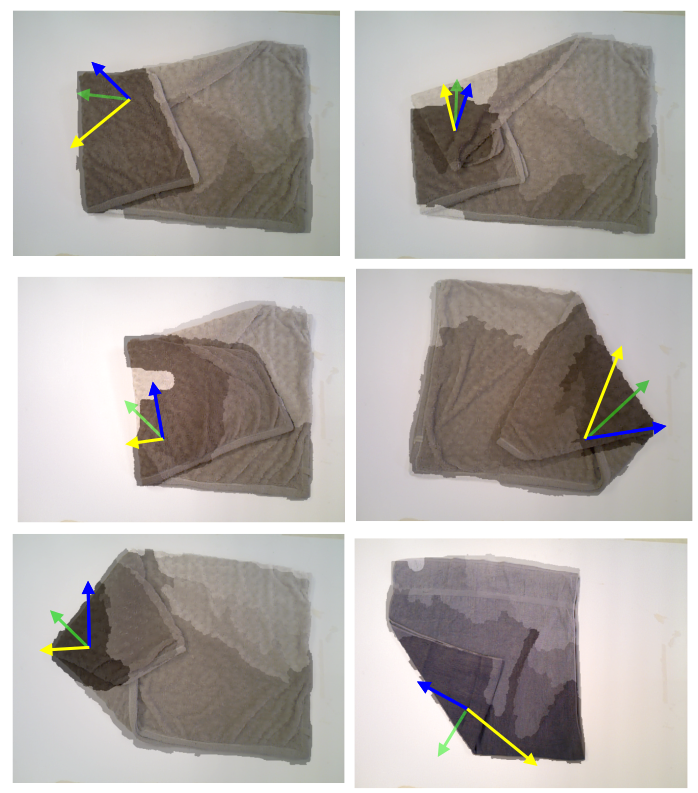
\includegraphics[width=0.8\textwidth]{figures/directions_several.png}
    \caption{Best directions calculated for each garment provided to the system. The direction with the smallest bumpiness value is shown in blue. The second best direction is shown in yellow. The bisector is shown in green. The arrows are for demonstrative purpose only, and their starting and ending point do not represent the pick and place point. The watershed computed regions are additionally overlaid upon the original image.}
    \label{directions_several}
\end{figure}

The final results show that the algorithm generates acceptable unfolding directions.
